\section{Web后端实现}

OJ的后端是基于Python和Django的,数据库使用MySQL,缓存及队列使用Redis和Celery。

\subsection{Django框架模块组成}

\subsubsection{Model数据库模型}
Model是数据模型,是Django ORM的重要组成部分。使用ORM可以大大简化数据库操作,提高开发效率,同时避免SQL注入等安全问题的发生。一般情况下一个Model映射到数据库中的一张表中,Model的每一个属性就是表中的每一个字段。比如说

\begin{verbatim}
class User(models.Model):
    username = models.CharField(max_length=64, unique=True, db_index=True)
    # 真实姓名
    real_name = models.CharField(max_length=30, blank=True, null=True)
    password = models.CharField(max_length=128)
    # 0是普通用户,管理员为1,超级管理员为2
    admin_type = models.IntegerField(default=0)
    email = models.EmailField(max_length=256, blank=True, null=True)
\end{verbatim}就会生成如下所示创建表的SQL语句。

\begin{verbatim}
CREATE TABLE user(
    id INT PRIMARY KEY,
    username VARCHAR(64) UNIQUE NOT NULL,
    real_name VARCHAR(30),
    password VARCHAR(128) NOT NULL,
    admin_type INT NOT NULL,
    email VARCHAR(256)
)
\end{verbatim}
如果需要创建用户名为foo的用户,可以使用\\\texttt{User.objects.create(username="foo", password="hidden", email="foo@gmail.com")}。如果需要查询用户名foo的用户,可以使用\texttt{user = User.objects.get(username="foo")},Django就会自动的将其转换为SQL语句\texttt{SELECT id, username, password, email FROM user WHERE username="foo";},然后就可以访问\texttt{user}对象的属性来获取具体字段的值。

如果需要修改用户信息,可以直接给属性赋值,然后调用\texttt{saeve}方法即可。比如
\begin{verbatim}
user.emai="foo@example.com"
user.save()
\end{verbatim}Django就可以生成对应的SQL update语句。

\subsubsection{View视图处理函数}

View视图处理函数就是业务逻辑所在了,负责处理各种请求、进行数据校验、与数据库进行交互和调用第三方API等。

Django的View处理函数都是与URL绑定的,符合该URL规则的请求就会进入对应的View函数处理。比如

\begin{verbatim}
url(r'^problem/(?P<problem_id>\d+)/$', "problem.views.problem_page")

def problem_page(request, problem_id):
    try:
        problem = Problem.objects.get(id=problem_id, visible=True)
    except Problem.DoesNotExist:
        return error_page(request, u"题目不存在")
    return render(request, "oj/problem/problem.html", {"problem": problem})
\end{verbatim}

View视图处理函数一般接收\texttt{request}和部分URL中匹配的值为参数,需要返回一个\texttt{HTTPResponse}对象。

\subsection{部分模块功能实现}
下面将以部分逻辑比较复杂的模块为例,详细分析OJ后端的开发过程。

\subsubsection{用户登录}
用户登录是几乎所有网站必备的基础功能。用户提交用户名和密码,然后数据POST到后端进行查询和验证,如果验证通过,就设置Cookies,否则提示用户名或密码错误。

\begin{verbatim}
class UserLoginAPIView(APIView):
    def post(self, request):
        """
        用户登录json api接口
        ---
        request_serializer: UserLoginSerializer
        """
        serializer = UserLoginSerializer(data=request.data)
        if serializer.is_valid():
            data = serializer.data
            user = auth.authenticate(username=data["username"], password=data["password"])
            # 用户名或密码错误的话 返回None
            if user:
                auth.login(request, user)
                return success_response(u"登录成功")
            else:
                return error_response(u"用户名或密码错误")
        else:
            return serializer_invalid_response(serializer)
\end{verbatim}

这里使用了Django Rest Framework的\texttt{APIView},可以简化通过AJAX和API通信的Web程序的开发,这里只实现了\texttt{POST}函数,如果不是\texttt{POST}方法请求API就会收到错误响应。

\texttt{serializer}是用来校验数据的,写法和Model类似,需要规定字段和对应的数据类型等,\texttt{UserLoginSerializer}的实现代码是

\begin{verbatim}
class UserLoginSerializer(serializers.Serializer):
    username = serializers.CharField(max_length=64)
    password = serializers.CharField(max_length=128)
\end{verbatim}

如果缺少字段或者字段的数据不符合要求,就会返回一个\\\texttt{serializer\_invalid\_response(serializer)}的响应,这是一个封装后的函数,实现代码是

\begin{verbatim}
def serializer_invalid_response(serializer):
    for k, v in serializer.errors.iteritems():
        return error_response(k + " : " + v[0])
\end{verbatim}

通过\texttt{serializer.errors}属性可以得到错误详情,然后返回前端,提示用户。

如果数据校验通过,就会使用用户名和密码作为参数,调用Django的\texttt{auth.authenticate}方法进行验证。\texttt{auth.authenticate}实现也比较简单,首先根据配置文件选择密码的哈希函数计算密码的哈希值,然后使用用户名和哈希值去数据库查询,如果查询到记录,说明用户名密码正确,返回对应的\texttt{User}对象。

因为HTTP协议是一个无状态的协议,服务器端需要通过Cookies来将请求和登录的用户进行对应,这个对应关系是保存在服务器端的,有时也称为\texttt{Session},这个过程就是\texttt{auth.login(request, user)}实现的。

Django生成的数据库中有\texttt{django\_session}表,表中有三个字段,\texttt{session\_key}、\texttt{session\_data}和\texttt{expire\_date}。首先Django会在这张表中插入一条记录,简化的demo如下。

\begin{verbatim}
DjangoSession.objects.create(session_key=random_string(), 
                             session_data=json.dumps({"user_id": user.id}), 
                             expire_date=some_date())
\end{verbatim}

然后使用\texttt{set-cookie} HTTP头给浏览器设置一个Cookie,比如\texttt{set-cookie:sessionid=\\9400de64wpdhtd8w5s82ntvy6ht3nsd5; expires=Wed, 18-May-2016 13:13:34 GMT; httponly; Max-Age=1209600; Path=/},key是\texttt{sessionid},value是数据库里的\texttt{session\_key},还包括过期时间等信息。

这样每次用户请求的时候,取到Cookies中\texttt{sessionid}的值,再去表中查询就可以得到当前用户的ID了。

\subsubsection{重置密码}

重置密码功能的设计关乎用户用户账户的安全,已经有很多案例说明重置密码功能设计缺陷带来的安全问题\cite{password-reset-vul}。

用户提交重置密码请求后,首先会查询邮箱是否存在,如果存在,就会生成32位长度的随机token和30分钟的过期时间。然后调用异步队列,向该邮箱发送重置密码链接,响应前端重置邮件已发出。

用户收到邮件之后,点击重置链接,后端会先验证该链接的有效性,包括是否存在和是否过期,如果验证通过就会返回重置密码页面。用户填写新密码提交后,会再次验证token的有效性,如果验证通过,就会查询该token对应的用户,然后更新密码。

\begin{figure}[H]
\centering
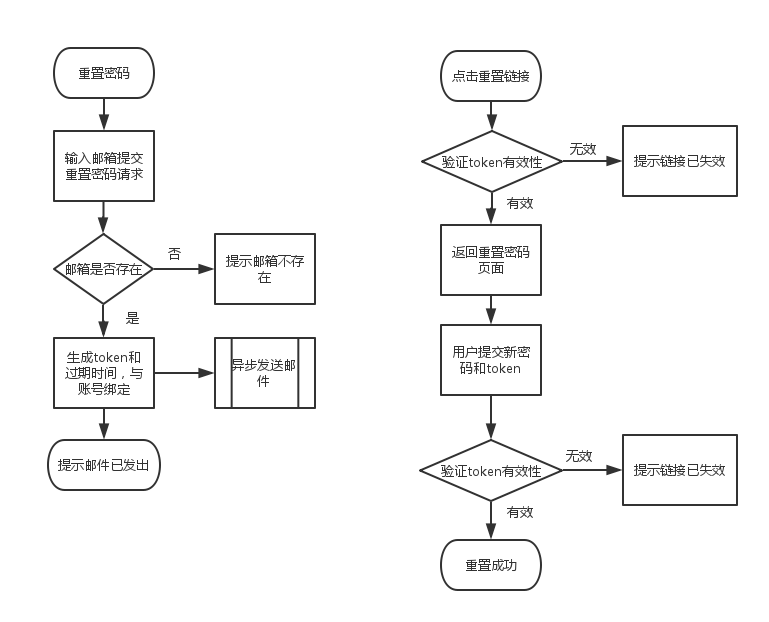
\includegraphics[width=0.6\textwidth]{password-reset-flow}
\caption{密码重置流程}
\end{figure}

\subsubsection{比赛排名}
比赛排名的Model是
\begin{verbatim}
class ContestRank(models.Model):
    user = models.ForeignKey(User)
    contest = models.ForeignKey(Contest)
    total_submission_number = models.IntegerField(default=0)
    total_ac_number = models.IntegerField(default=0)
    total_time = models.IntegerField(default=0)
    submission_info = JSONField(default={})
\end{verbatim}

可以看到,记录了具体题目提交信息的字段保存的是JSON数据,格式是\texttt{\{\$problem\_id: \{"is\_ac": True/False, "ac\_time": \$ac\_time, "error\_number":\$error\_number, \\"is\_first\_ac": True/False\}\}}这样可以简化数据库设计的难度,让SQL数据库按照NoSQL来用。这样每一个用户就是一条记录,也就是排名上的一行。只要根据\texttt{contest\_id}查询一次数据库后,就可以得到生成页面的全部数据。

鉴于比赛参与人数可能很多,排名数据偏大,如果每次重新生成,可能会遇到性能问题,我们在这里使用了Redis作为缓存,在HUSTOJ等系统中也有类似的用法\cite{hustoj-cache}。使用\texttt{\$\{contest\_id\}\_rank\_cache}作为缓存的key。每次生成页面的时候,先使用缓存key去Redis中取数据,如果没有取到,就去MySQL中查询,同时生成Redis缓存。每次有新的提交的时候,异步队列需要主动的清除Redis缓存,避免页面数据过期。
\subsection{判题模块}

\subsubsection{选择判题服务器}
在OJ使用人数较多的情况下,需要使用多台服务器进行判题。选择哪一台服务器,怎么均衡服务器负载,怎么与服务器通信、怎么得到服务器判题结果就是我们要面对的问题了。

管理员可以在admin后台配置多台判题服务器,每台服务器都有自己的最大判题实例数量\texttt{max\_instance\_number}、当前使用的判题实例数量\texttt{used\_instance\_number}和负载\texttt{workload}三个指标,每次分配给该服务器一个判题任务,当前已经使用的实例数加一,服务器的负载workload就会修改为${\frac {used\_instance\_number}{max\_instance\_number}} \times 100$ \%,判题结束的时候,当前已经使用的实例数减一,负载值也对应修改。分配给该服务器同时运行的任务不会超过该服务器的最大判题实例的值。

\subsubsection{RPC通信}
XML-RPC是一个远程过程调用(remote procedure call,RPC)的分布式计算协议,通过XML将调用远程机器上的函数封装,一般使用HTTP协议作为通信协议。

在远程机器上启动XML-RPC Server,注册\texttt{JudgeInstanceRunner}类,供远程调用。

\begin{verbatim}
server = AsyncXMLRPCServer(('0.0.0.0', 8080), SimpleXMLRPCRequestHandler)
server.register_instance(JudgeInstanceRunner())
server.serve_forever()
\end{verbatim}

由上一部分选择好服务器后,指定服务器的IP和端口就可以运行代码了。

\begin{verbatim}
s = TimeoutServerProxy("http://" + judge_server.ip + 
                             ":" + str(judge_server.port), timeout=30)
data = s.run(judge_server.token, self.submission.id, self.submission.language,
             self.submission.code, self.time_limit, self.memory_limit, 
             self.test_case_id, self.spj, self.spj_language,
             self.spj_code, self.spj_version)
\end{verbatim}

\subsubsection{用户代码的运行过程}
在判题服务器上,有对应语言的编译参数和运行参数配置。以下是C语言的编译和运行参数。

\begin{verbatim}
{
    "name": "c",
    "src_name": "main.c",
    "code": 1,
    "compile_max_cpu_time": 3000,
    "compile_max_memory": 128 * 1024 * 1024,
    "compile_command": "/usr/bin/gcc -DONLINE_JUDGE -O2 \
                        -w -fmax-errors=3 -std=c99 {src_path} -lm -o {exe_path}/main",
    "spj_compile_command": "/usr/bin/gcc -DONLINE_JUDGE -O2 \
                            -Werror -fmax-errors=3 -std=c99 {src_path} -lm -o {exe_path}",
    "execute_command": "{exe_path}/main",
    "use_sandbox": True
}
\end{verbatim}

首先按照参数编译用户代码,可执行文件存放在指定的目录。如果出现编译错误或者编译器异常,直接返回错误信息,提示编译错误。如果编译通过,将会在沙箱中运行用户代码,\texttt{stdin}的输入来自于上传的测试用例文件重定向,进程的\texttt{stdout}会重定向到指定的输出文件。

进程正常结束后,系统将会计算重定向输出文件去除最后的空格和换行后的md5,与上传的测试用例的md5(这些数据已经保存在文件的meta信息中了)进行比较,如果一致,说明测试通过,否则是答案错误。

如果进程非正常结束,会返回运行错误等信息。这些细节将在后文判题沙箱中详述。

如果这个提交对应的题目是Special Judge类型,那上面的判断过程是由出题人上传的代码来执行的。每个Special Judge都有一个版本号,每次更新后会变。如果发现目录中没有当前版本号的SPJ程序,系统就会先编译SPJ的代码,这样就解决了更新SPJ代码后无法重新编译的问题。

SPJ代码需要按照一定的模板来写,测试用例文件和用户输出文件的路径将会作为两个参数传递给Special Judge,然后通过进程返回值来获取判题结果。

\subsubsection{判题结束后的各种动作}

服务器判题结束后,还有一系列的动作需要执行,包括:

\begin{itemize}
    \item[-] 更新题目提交数量和AC数量计数器
    \item[-] 更新用户做题状态计数器,用于题目前面显示对应的符号
    \item[-] 更新用户做题数量和AC数量计数器
    \item[-] 比赛排名缓存的刷新
\end{itemize}

\subsection{Virtual Judge的实现}

\subsubsection{简介}

Virtual Judge是一种特殊的OJ系统。与其他OJ系统不同的是,Virtual Judge系统本身并没有任何测试数据,而是通过在其他OJ系统中的机器人账号进行测试并抓取测试结果。因此可以在只有题目而没有测试数据的前提下建立竞赛。\cite{wiki-vj}

\subsubsection{插件式爬虫}

对于每个OJ,具体的处理方法和过程都是不同的,但是最终要实现的功能都是统一的,比如登录用户、获取指定URL的题目、提交题目和获取指定的提交结果。在这种情况下,我们可以让每个OJ的爬虫都继承一个父类,需要实现父类中所有的公开方法,如果子类没有实现该方法,调用的时候就会引发\texttt{NotImplementedError}异常。

\begin{figure}[H]
\centering
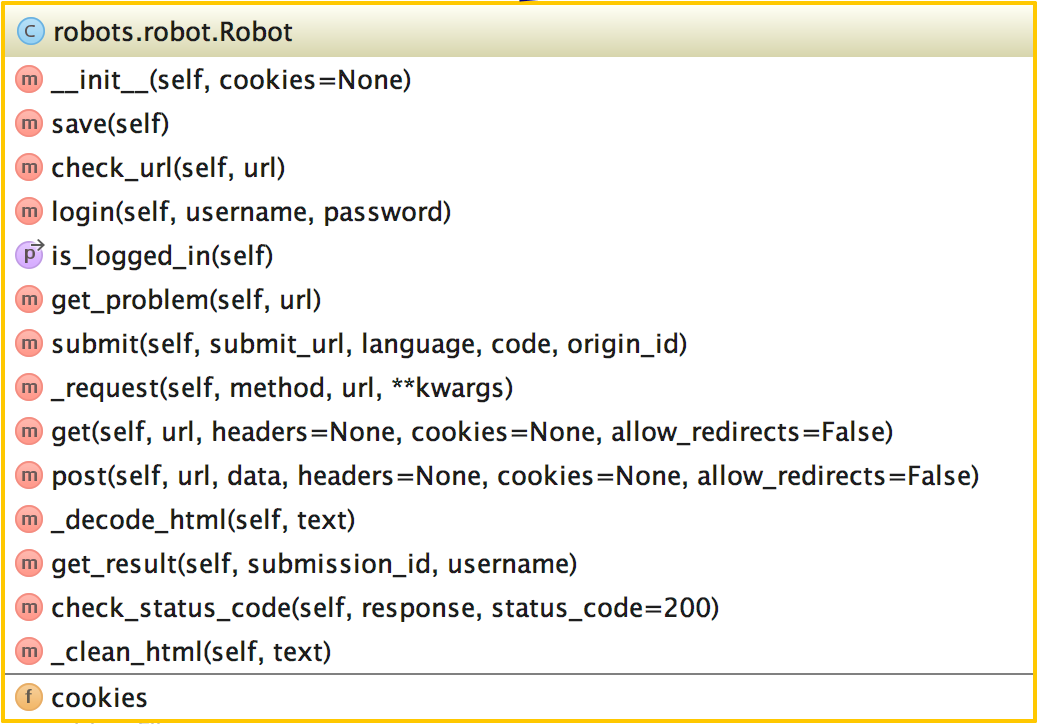
\includegraphics[width=0.6\textwidth]{robot-uml}
\caption{爬虫父类的UML}
\end{figure}

部分函数的作用:
\begin{itemize}
    \item[-] \texttt{save}:返回登陆后Cookies和token信息
    \item[-] \texttt{check\_url}:检查是否是本OJ题目的URL
    \item[-] \texttt{login}:使用给定的用户名密码登录OJ
    \item[-] \texttt{get\_problem}:获取指定URL的题目信息
    \item[-] \texttt{submit}:提交题目
    \item[-] \texttt{get}和\texttt{post}:HTTP协议请求网络
    \item[-] \texttt{get\_result}:获取提交结果
\end{itemize}

\subsubsection{工作流程}

以获取杭州电子科技大学OJ题目详情为例,具体实现的逻辑是:

\begin{verbatim}
def get_problem(self, url):
    if not self.check_url(url):
        raise RequestFailed("Invaild Hduoj url")
    regex = {"title": r"<h1 style='color:#1A5CC8'>(.*)</h1>",
             "time_limit": r"Time Limit:\s*[\d]*/([\d]*)\s*MS",
             "memory_limit": r"Memory Limit:\s*[\d]*/([\d]*)\s*K",
             "description": r"Problem Description</div>\s*
                              <div class=panel_content>([\s\S]*?)</div>",
             "input_description": r"Input</div>\s*
                                    <div class=panel_content>([\s\S]*?)</div>",
             "output_description": r"Output</div>\s*
                                     <div class=panel_content>([\s\S]*?)</div>",
             "hint": r"Hint(?:[\s\S]*?Hint[\s\S]*?</i>|
                       </i>\s*</div>)([\s\S]*?)</div>",
             "spj": r"<font color=red>Special Judge</font>",
             "samples": r'Courier New,Courier,monospace;">([\s\S]*?)(?:<div|</div>)'}
    problem_id = re.compile(r"\d{4}").search(url).group()
    data = self._regex_page(url, regex)
    data["id"] = problem_id
    data["submit_url"] = "http://acm.hdu.edu.cn/submit.php?action=submit"
    return data
\end{verbatim}

以提交题目并获取提交结果为例,分析爬虫提交题目的的工作逻辑。此步骤涉及到多个异步任务。

首先根据请求数据中的题目id获取给题目对应的OJ的具体信息,在VJ数据库中创建该提交的记录,查询当前是否有空闲的爬虫用户用于提交。

如果没有空闲的爬虫用户,该提交就会被放入一个等待队列中,返回提交信息,否则将会修改该用户的标志位,设置为被占用。

然后会根据OJ的设置和该用户的登录信息实例化一个对应的爬虫,传递所需参数,创建\texttt{submit\_dispatcher}异步任务,得到\texttt{task\_id},更新到数据库,返回调用者提交信息。这时,爬虫在后端异步的运行。

而\texttt{submit\_dispatcher}异步任务会去创建真正的提交异步任务\texttt{submit},同时还会设置该异步任务的回调函数为\texttt{submit\_waiting\_submission}和\texttt{update\_submission},然后将该\texttt{task\_id}更新到数据库中。

\texttt{submit}方法会调用爬虫的\texttt{submit}方法去提交代码,接着循环请求判题结果,直到得到结果或者超过最多尝试次数,最终返回结果。

等到\texttt{submit}执行完毕的时候,两个回调函数会被调用,功能分别是提交等待队列中的题目和更新该次提交的信息。如果等待队列中没有提交,就会释放该爬虫用户,否则直接使用该用户继续提交题目,回到本流程开头。

\subsection{安全问题}

\subsubsection{用户密码存储}

现代网站已经不再使用明文密码存储的方式了,而是改用只在数据库中存储明文密码的哈希。常见的哈希算法有MD5和SHA,可以从任何一段字符串计算出一段固定长度的哈希值。这样当用户输入密码时,直接将该密码代入算法得出哈希值,再与存储的哈希值对比,相同则允许登录。用户注册时也是直接存储密码的哈希值,而不是明文密码。这样就防止数据库泄露的时候导致用户明文密码泄露。

但是随着计算能力大幅提高,MD5和SHA1算法已经不再推荐使用了,这些算法被碰撞的几率已经越来越大了。本系统中存储密码使用的Django默认哈希方法,SHA256加salt后使用PBKDF2算法处理,该算法计算消耗的CPU时间非常多,能大大减慢暴力破解速度。

\subsubsection{XSS}

XSS漏洞跨站脚本攻击,是Web程序中常见的漏洞。其原理是攻击者向有XSS漏洞的网站中传入恶意的HTML和JavaScript代码,当其它用户浏览该网站时,JavaScript代码会自动执行,从而达到攻击的目的。比如盗取用户Cookie、重定向到其它网站等。

Django模板默认对模板输出全部转义,避免了绝大多数的XSS问题。但是有一些输出是不能转义的,比如公告的内容、题目的说明等,它们是使用富文本编辑器进行编辑的,如果进行过滤,文字的样式就无法显示了。所以我们在这里需要过滤危险的JavaScript和HTML属性等,使用了https://github.com/phith0n/python-xss-filter作为过滤器。

\subsubsection{SQL注入}

SQL注入攻击,是Web开发中最常见的一种安全漏洞。可以用它来从数据库获取敏感信息,甚至有可能获取数据库乃至系统用户最高权限。而造成SQL注入的原因是因为程序没有有效过滤用户的输入,使攻击者成功的向服务器提交恶意的SQL查询代码,程序在接收后错误的将攻击者的输入作为查询语句的一部分执行,导致原始的查询逻辑被改变,额外的执行了攻击者的代码。

OJ系统全部使用Django的ORM进行数据库查询,而ORM在进行查询的时候使用了SQL参数绑定,所以不存在SQL注入的风险。

\subsubsection{CSRF}

CSRF可以伪造受信任用户的请求来利用受信任的网站。攻击者可以在第三方网站hacker.com设置代码,用户在浏览这些网页的时候向victim.com跨域发送数据,浏览器根据同源策略,带上了victim.com的cookies,导致请求被伪造,可能造成很大的危害,比如发送微博、添加管理员、修改密码等。

OJ系统采取的措施是需要修改服务器状态的请求全部增加token验证,token是在Cookies中读取的,而根据同源策略,hacker.com是无法读取victim.com的Cookies的,这样就无法伪造token。后端服务器只要对比Cookies中的token和请求头中的token是否一致就可以了。

\subsubsection{沙箱安全}

沙箱安全是整体开发中的重点和难点,本文将在第5章中详细分析。
     
\subsubsection{其他安全问题}

上面提到的几个安全问题是出现频率比较高的,危害比较大的。还有一些其他的安全问题没有单独列出,比如密码暴力破解、恶意提交请求等。

针对密码暴力破解,增加了管理员密码的两步验证。管理员在登录的时候,必须同时输入手机动态密码app上显示的验证码。针对恶意注册,增加了验证码。

针对使用脚本进行大量恶意提交的问题,使用Token Bucket机制增加了频率限制,同时为一定的并发请求预留了空间。当用户触发频率限制的时候,将会得到提交失败的提示和需要等待的时间。
